\documentclass[11pt]{article}
\usepackage[english]{babel}
\usepackage[utf8x]{inputenc}
\usepackage{amsmath}
\usepackage{graphicx}
\usepackage{float}
\usepackage[colorinlistoftodos]{todonotes}
\usepackage[T1]{fontenc}
\usepackage{listings}
\def\code{\lstinline[basicstyle=\ttfamily]}
%\usepackage[margin=0cm]{geometry}
\usepackage{hyperref}
\usepackage{algorithm}
\usepackage{algorithmic}
\usepackage{xcolor}

\definecolor{mGreen}{rgb}{0,0.6,0}
\definecolor{mGray}{rgb}{0.5,0.5,0.5}
\definecolor{mPurple}{rgb}{0.58,0,0.82}
\definecolor{backgroundColour}{rgb}{0.95,0.95,0.92}

\lstdefinestyle{cstyle}{
    backgroundcolor=\color{backgroundColour},   
    commentstyle=\color{mGreen},
    keywordstyle=\color{magenta},
    numberstyle=\tiny\color{mGray},
    stringstyle=\color{mPurple},
    basicstyle=\footnotesize\ttfamily,
    breakatwhitespace=false,         
    breaklines=true,                 
    captionpos=b,                    
    keepspaces=true,                 
    numbers=left,                    
    numbersep=5pt,                  
    showspaces=false,                
    showstringspaces=false,
    showtabs=false,                  
    tabsize=4,
    language=C
}


\begin{document}

\begin{titlepage}

\newcommand{\HRule}{\rule{\linewidth}{0.5mm}} % Defines a new command for the horizontal lines, change thickness here

\center % Center everything on the page
 
%----------------------------------------------------------------------------------------
%	HEADING SECTIONS
%----------------------------------------------------------------------------------------

\textsc{\LARGE Paris Diderot University}\\[1.5cm]
\textsc{\Large Engineering School Denis Diderot}\\[0.5cm] 

%----------------------------------------------------------------------------------------
%	TITLE SECTION
%----------------------------------------------------------------------------------------


\HRule \\[0.4cm]
{ \huge \bfseries Dynamic Memory Allocation in C}\\[0.4cm] 
\HRule \\[1.5cm]
 
 \textsc{\large second year internship report}\\[1.5cm] 
%----------------------------------------------------------------------------------------
%	AUTHOR SECTION
%----------------------------------------------------------------------------------------

\begin{minipage}{0.4\textwidth}
\begin{flushleft} \large
\emph{Author:}\\
Mamadou Yéro \textsc{Baldé} % Your name
\end{flushleft}
\end{minipage}
~
\begin{minipage}{0.4\textwidth}
\begin{flushright} \large
\emph{Supervisor:} \\
Mihaela \textsc{Sighireanu} % Supervisor's Name
\end{flushright}
\end{minipage}\\[2cm]

%----------------------------------------------------------------------------------------
%	DATE SECTION
%----------------------------------------------------------------------------------------

{\large \today}\\[0.1cm] % Date, change the \today to a set date if you want to be precise

%----------------------------------------------------------------------------------------
%	LOGO SECTION
%----------------------------------------------------------------------------------------


\includegraphics[width=0.5\textwidth]{figures/eidd.jpeg}\\[0cm] % Include a department/university logo - this will require the graphic package
 
%----------------------------------------------------------------------------------------

\vfill % Fill the rest of the page with whitespace

\end{titlepage}

Les allocateurs de memoire dynamique gèrent le tas (\emph{heap}) d'un program.
Ils sont indispensables à tout langage de programmation moderne. En C, l'allocateur de memoire est inclu dans la bibliothèque standard; en Java, il fait partie de l'environnement d'exécution (\emph{runtime}).
Le code de ces allocateurs est assez petit, mais il est notoirement difficile à mettre au point car il doit utiliser des primitives de programmation complexes: arithmetique des pointeurs, operations bit à bit, appels système. De plus, les structures de données que ce code utilise sont assez complexes: liste-tas (champs suivant obtenu avec l'arithmetique des pointeurs), listes doublement chainées, listes circulaires, arbres binaires de recherche, tables de hachage. 

Pour mettre au point ces programmes, des techniques de verification formelles ont été developpées par l'équipe ``Modélisation et Vérification'' de l'IRIF, où mon stage a eu lieu. Ces techniques sont basées sur des logiques de programmes. Mon travail a été de fournir des programmes de test pour ces techniques.
J'ai donc mis au point quatre allocateurs en utilisant des techniques de test unitaire et en s'appuyant sur la  bibliotheque CUNIT.
%%%%%%%%%%%%%%%%%%%%%%%%%%%%%
\clearpage

\tableofcontents

%----------------------------------------------------------------------------------------
%	Report CONTENT - CHAPTERS
%----------------------------------------------------------------------------------------
%----------------------------------------------------------------------------------------
%	INTRODUCTION SECTION
%----------------------------------------------------------------------------------------
\section{Introduction}
\label{sec:introduction}

Context du stage, que as tu fait, ou, quand, resultats.

la suite dans l'entete du chapitre 2

Memory allocation is mainly a computer hardware operation which is managed through operating system and software applications. Its process is pretty similar to the physical and virtual memory management. Programs and services are assigned with a specific memory as per their requirements when they are executed. Once the program has finished its operation or is idle, the memory is released and allocated to another program or merged within the primary memory.\\

Memory allocation has two core types:
\begin{itemize}
\item Static Memory Allocation: The program is allocated memory at compile time.
\end{itemize}

\begin{itemize}
\item Dynamic Memory Allocation: The programs are allocated with memory at run time.
\end{itemize}

In this report, we will focus on the dynamic allocation of memory and its operation.

%----------------------------------------------------------------------------------------
%	Presentation of IRIF SECTION
%----------------------------------------------------------------------------------------

\subsection{Presentation of IRIF}
\textbf{Research Institute on the Foundations of Computer Science }
(IRIF) is a research unit co-founded by the CNRS and the University Paris-Diderot, as UMR 8243. IRIF hosts two INRIA project-teams. IRIF is also member of the Foundation of Mathematical Sciences of Paris (FSMP) and of the Federation of Research in Mathematics of Paris. \\

IRIF results from the merging of the two research units LIAFA and PPS on January 1st, 2016. The scientific objectives of IRIF are at the core of computer science and, in particular, they focus on the conception, analysis, proof, and verification of algorithms, programs, and programming languages. They are built upon fundamental research activities developed at IRIF on combinatorics, graphs, logics, automata, type, semantics, and algebras.\\

At the CNRS, IRIF is primarily affiliated to the Institute of Computer Science (INS2I), and, secondarily, to the Institute of Mathematics (INSMI). IRIF is part of the Department of Computer Science of the University Paris-Diderot, and also hosts several members of the Department of Mathematics. Last, IRIF is affiliated to the doctoral school of Mathematical Sciences of Paris (ED 386).\\ 

IRIF is structured in nine thematic teams, grouped into three research poles: 
\begin{itemize}
\item Pole Algorithms and discrete structures:

\begin{itemize}
\item Algorithms and complexity
\end{itemize}

\begin{itemize}
\item Combinatorics
\end{itemize}

\begin{itemize}
\item Complex Systems, Networks, and Distributed Computing 
\end{itemize}

\begin{itemize}
\item Theory and algorithmics of graphs 
\end{itemize}

\end{itemize}

\begin{itemize}
\item Pole Automata, structures and verification:

\begin{itemize}
\item Automata and applications
\end{itemize}
\begin{itemize}
\item Modeling and verification
\end{itemize}

\end{itemize}

\begin{itemize}
\item Pole Proofs, programs and systems:
\begin{itemize}
\item Algebra and computation
\end{itemize}
\begin{itemize}
\item Analysis and conception of systems 
\end{itemize}
\begin{itemize}
\item Proofs and programs
\end{itemize}

\end{itemize}
IRIF hosts currently a hundred permanent members), including roughly 54 faculty members, 30 CNRS researchers, 6 INRIA researchers and 5 administrative and technical staffs (in January 2018). The total number of IRIF members, including PhD students, post-docs, and long-term visitors amounts for about two hundred. \\

I've done my internship the the ``modeling and verification'' team, which studies and develops methods and tools for the software verification.


%----------------------------------------------------------------------------------------
%	Motivation SECTION
%----------------------------------------------------------------------------------------
\subsection{Motivation}

les allocateurs sont des programmes petits mais tres difficiles à mettre au point car ils appellent des primitives de programmation complexes: arithmetiques de pointeur, operations bit à bit, appels aux systeme (pour etendre la memoire du processus). De plus, les structures de données sont assez complexes: heap-listes (chnamps next obtenu avec arithmetique de pointeur), listes doublement chainées, circulaires, arbres binaires de rechrche, table de hashage. 

Pour mettre au point ce programmes, des techniques de verification formelles ont été developpées. Ces techniques sont basées sur des logiques de programmes (logique de Hoare). Mon travail a fournit des programmes de test de ces techniques.


Dans mon stage j'ai mis au point ces allocateurs en utilisant du test unitaire et la  bibliotheque CUNIT.


%----------------------------------------------------------------------------------------
%	SECTION
%----------------------------------------------------------------------------------------
\section{Heap and System Calls}
\label{sec:heap}

In the order to understand dynamic memory allocation, we need to understand how the memory of a process executing a program is handled in most operating systems. We will keep an abstract point of view for that part, since many details are operating system and
hardware dependent.

\subsection{The Process’s Memory}
Every process has its own virtual address space which is dynamically translated into physical memory  address space by the memory management unit (MMU) and the kernel. This memory space may be seen as a contiguous array of bites, like in Figure~\ref{fig:memory}. It is divided in several parts, mainly:
\begin{itemize}
\item the text part containing the code executed,
\item the data part space for constant and global variables,
\item the stack where local variables of functions called during the process execution are stored, and 
\item the program’s data created during the execution, called the \emph{heap}.
\end{itemize}

The DMA manages the heap. The heap is a continuous (in terms of virtual addresses) space of memory blocks with three bounds (see Figure~\ref{fig:memory}): 
a starting point, 
a maximum limit (managed through \code{sys/resource.h}’s functions \code{getrlimit()} and \code{setrlimit()}) and 
an end point called the break. The break marks the end of the used memory space, that is, the part of the heap that is managed by the dynamic allocation \cite{WilsonJNB95}.

\begin{figure}[htbp]
    \begin{center}
        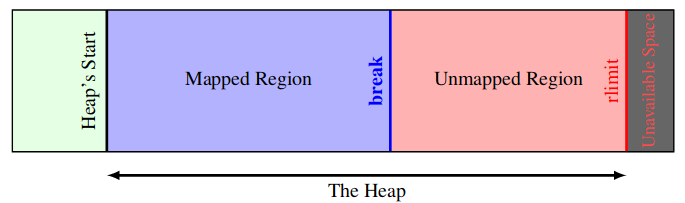
\includegraphics[width=0.8\textwidth]{figures/heap}
    \caption{Memory organization}
    \label{fig:memory}
    \end{center}
\end{figure}


\subsection{System Calls}

To manage the heap, the DMA calls low level primitives of the operating system in order to obtain the starting point of the heap and the break point position; it also needs to be able to move the break point.
For the Unix systems, these primitives are \code{brk()} and \code{sbrk()}, whose signature is:
\begin{lstlisting}[style=cstyle]
int brk(const void *addr);
void* sbrk(intptr_t incr);
\end{lstlisting}

As specified by the Unix manual, \code{brk()} and \code{sbrk()} change the location of the break point. Increasing the break point has the effect of allocating heap memory to the process; decreasing the break deallocates memory.

\code{brk()} sets the break point to the value specified by \code{addr}, when that value is reasonable, the system has enough memory, and the process does not exceed its maximum more limit.

\code{sbrk()} increments the break point by \code{incr} bytes, with the same limitations like above. Calling \code{sbrk()} with an increment of 0 can be used to find the current location of the program break.

On success, \code{brk()} returns zero. On error, \code{-1} is returned. %, and \code{errno} is set to \code{ENOMEM}.
%
On success, \code{sbrk()} returns the previous program break. (If the break was increased, then this value is a pointer to the start of the newly allocated memory). On error, \code{(void *) -1} is returned. %, and \code{errno} is set to \code{ENOMEM}.\\


\subsection{Heap Initialization}

Using these system calls, the DMA starts from a initial size of the heap and moves the break depending on the client's needs. The initial configuration of the heap region may be fixed to some \code{size} using the following code,
where the global variables \code{hit} and \code{hli} denote the start respectively the limit (first after the last) address of the memory region managed:

\begin{lstlisting}[style=cstyle]
void minit(int size) 
{ hst=sbrk(size); hli=sbrk(0); }
\end{lstlisting}

Figure~\ref{fig:init} illustrates the heap region obtained with the above code.
In this region, the DMA manages its own data and the data allocated for the process.
 
\begin{figure}[htbp]
    \begin{center}
        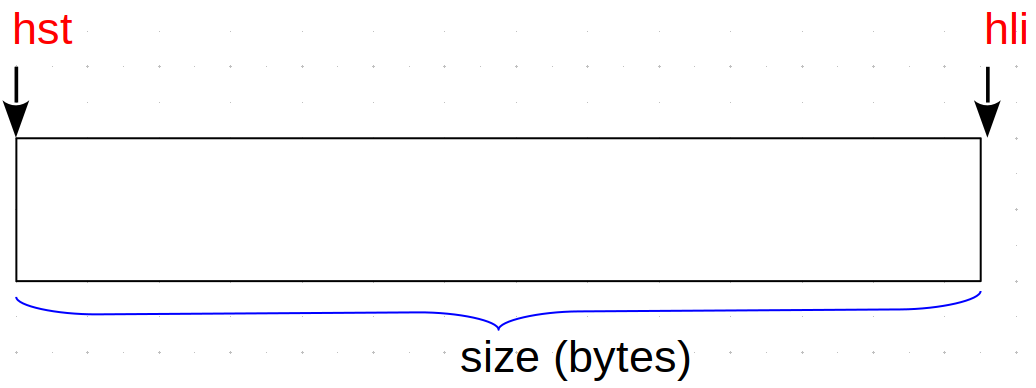
\includegraphics[width=0.6\textwidth]{figures/sbrk}
    \caption{Initial configuration of the heap}
    \label{fig:init}
    \end{center}
\end{figure}




%----------------------------------------------------------------------------------------
%	SECTION
%----------------------------------------------------------------------------------------

\section{Dynamic Memory Allocation}
\label{sec:dma}

We focus on this work on the DMA for the C language.

\subsection{User interface}

Usually, programs use the dynamic memory allocation to add a node to a data structure whose size is not known. In object oriented languages, dynamic memory allocation is used to get the memory for a new object, for example the primitive \code{new} in Java. The program may ask for memory of different sizes at different execution points.

Memory allocated may be returned whenever it is no longer needed. Memory can be returned in any order without any relation to the order in which it was allocated. 

Two functions make it possible to reserve and release dynamically an area of memory: \code{malloc()} for the reservation and \code{free()} for the liberation of previously allocated memory via \code{malloc()}.

\subsubsection{Memory allocation}
\code{malloc} is a C standard library function which is used to allocate a block of memory on the heap. The program accesses this block of memory via a pointer that \code{malloc} returns.
The function signature is:

\begin{lstlisting}[style=cstyle]
void* malloc(size_t size);
\end{lstlisting}

The only parameter to pass to malloc is \code{size}, the \emph{number of bytes} to allocate. The returned value is the address of the first byte of the allocated memory area. If the allocation could not be realized (due to lack of free memory), the return value is the \code{NULL} constant.

\subsubsection{Memory release}
When memory returned by \code{malloc()} is no longer useful, it doesn't get freed on its own. In the order to release the space allocated before, the program should explicitly use another C standard library function: \code{free()}.
The function signature is:
\begin{lstlisting}[style=cstyle]
void free(void *ptr);
\end{lstlisting}
\code{free()} releases the memory space pointed by \code{ptr}, which shall be a pointer obtained on a previous call to \code{malloc()}. If \code{ptr} has already been released, the behavior of \code{free()} is undetermined and it is considered a programming flaw. If \code{ptr} is \code{NULL}, no attempt to release takes place.


\subsubsection{Memory fragmentation}
The heap region managed by the DMA (see Figure~\ref{fig:init}) is initially considered free  and may be allocated entirely by a call to \code{malloc} of the size nearly equal to \code{size}.
However, programs are usually asking for smaller blocks, which are reserved by splitting the  heap region managed by the DMA in several \emph{chunks}. I will present the precise organization of a chunk in the next section.

What is important here is to know that a chunk stores the block of memory required by the program and some internal data used by the DMA to manage the chunk.

With this splitting in chunks, the heap region may develop ``holes'' where previously allocated memory has been returned between blocks of memory still in use.
A new request for memory might return a range of addresses out of one of the holes. But it might not use up all the hole, so further dynamic requests might be satisfied out of the original hole.

If too many small holes develop, memory is wasted because the total memory used by the holes may be large, but the holes cannot be used to satisfy dynamic requests. This situation is called \emph{memory fragmentation} \cite{Knuth73a}. 

\subsection{Properties of good allocators}
An allocator must keep tracking chunks which are in use and free.
The main goals of a good allocator are \cite{Lea12}:
\begin{itemize}
\item Maximizing compatibility: The implemented allocator must be compatible with ANSI/POSIX conventions.
\item Maximizing portability: The allocator must cover as many systems as possible.
\item Minimizing space: The allocator shouldn't waste space and track contiguous chunk to minimize fragmentation.
\item Minimizing time: The time for allocation and release of memory should be as short as possible.
\item Maximizing tunability: Optional features and behavior should be controllable by users either statically (via \code{#define} and the like) or dynamically (via control commands such as \code{mallopt}).
\item Maximizing locality: Allocate chunks of memory that are typically used together near each other. This helps minimize page and cache misses during program execution.
\item Maximizing error detection: Ensure that the use of the allocator is safe by checking the parameters received. 
Also, it does not seem possible for a general-purpose allocator to also serve as general-purpose memory error testing tool such as Purify. However, allocators should provide some means for detecting corruption due to overwriting memory, multiple frees, and so on.
\end{itemize}



%----------------------------------------------------------------------------------------
%	SECTION
%----------------------------------------------------------------------------------------

\section{Implementing an Allocator}
\label{sec:impl}
Allocators are categorized by the mechanisms they use to keep track of free chunks and to coalesce neighboring free chunks.
In what follows, I will explain step by step the design principles of a class of allocators that manages free chunks using a list.

\subsection{Chunk Information}
At the beginning of every chunk, the DMA stores extra-informations, called meta-data (see Figure~\ref{fig:chunkrep}), about
the size of the chunk, a flag to mark free chunks (free or busy), the pointer to the next or previous free chunk. 
the pointer returned by \code{malloc} is the address in the chunk after this meta-data, that we call \emph{chunk header} in the following.

\begin{figure}[htbp]
    \begin{center}
        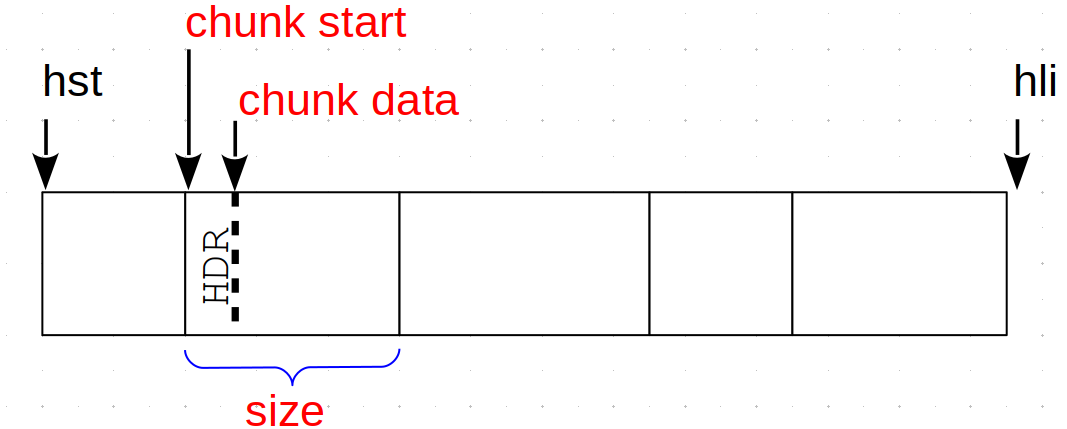
\includegraphics[width=0.8\textwidth]{figures/chunk}
    \caption{Chunk's internals}
    \label{fig:chunkrep}
    \end{center}
\end{figure}

There is a balance to find between the size of information stored in the meta-data and the memory consumption.
More information may lead to faster algorithms, but also reduces the available memory.
Let us present several ways of defining chunk header.

A chunk header storing the full information can be defining using the following C structure:
\begin{lstlisting}[style=cstyle]
typedef struct header
{
  size_t size;
  bool isfree;
  struct header *fpr;
  struct header *fnx;
} header;
\end{lstlisting}
where the field \code{size} stores the size in bytes of the full chunk (including the header), \code{is free} is the flag storing the status of the chunk, and \code{fpr} resp. \code{fnx} are used to implement the list of free chunks (and they are valid only if \code{isfree} is true).

A more compact solution for the header may be obtained if the flag for the chunk's status is stored with the size information. This is possible if the DMA maintains only chunks of even size. Therefore, the least significative bit of the size is always zero and may be used to store the flag on the status of the chunk.
Also, the list of free chunks may be only singly linked, therefore the \code{fpr} field may be eliminated.
The following definition implements this more compact solution:
\begin{lstlisting}[style=cstyle]
typedef struct header
{
  size_t size;			
  struct header *fnx;
} header;
\end{lstlisting}
and it will be used in the next section in the code I've implemented.
Notice that we can get the chunk size by doing a bitwise operation. 
The following chunk in the heap region is obtained by summing the address of the current chunk and the size of the chunk. The following macro-definitions get or set the information of the header defined above.
\begin{lstlisting}[style=cstyle]
// methods to get header information
#define HDR_GET_SIZE(p)     (p->size & (~1))
#define HDR_GET_STATUS(p)   (p->size & 1)
#define HDR_GET_NEXT(p)     ((header*) p + HDR_GET_SIZE(p))
#define HDR_SET_SIZE(p,nh)  p->size = (((nh + 1) >> 1) << 1) & (~HDR_GET_STATUS(p))
#define HDR_SET_STATUS(p)   p->size = p->size | 1
#define HDR_UNSET_STATUS(p) p->size = p->size & (~1)
\end{lstlisting}

The most compact solution is the one storing only an integer (4 bytes) as header. This integer may store the size of the chunk and the flag (as explained above), or the next pointer and the flag (if the addresses of chunks are always even).
The free list is not kept, which means that the DMA has to scan all the chunks to find the free ones and therefore is slower.
The following definition implements this very compact solution:
\begin{lstlisting}[style=cstyle]
typedef int header;
\end{lstlisting}


\subsection{Allocation Algorithms}
One of the important part of \code{malloc} is the way that free chunks are found and allocated. In what follows, we will discuss some policies and algorithms used to perform a dynamic allocation when the free chunks are stored in a list.
Figure~\ref{fig:freelist} illustrates a heap region managed by the DMA with free list.

\begin{figure}[htbp]
    \begin{center}
        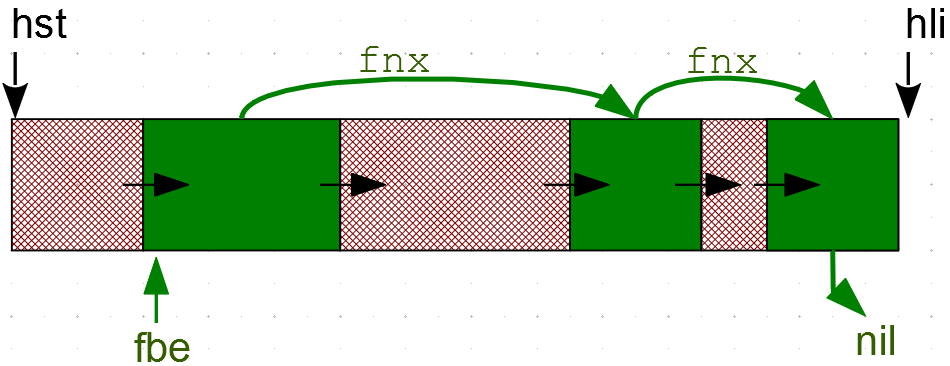
\includegraphics[width=0.8\textwidth]{figures/freelist}
    \caption{Heap with free list in green}
    \label{fig:freelist}
    \end{center}
\end{figure}

%First-fit method
\subsubsection{First-fit method}
The first-fit method allocates the first free chunk in the free list which has sufficient size to satisfy the request. If such a chunk does not exist, there are several choices.
In lazy allocators, a coalescing of neighboring free chunks is done, and then the DMA tries again to find a suitable free chunk.
Otherwise, if the break point does not reached the heap limit, the DMA has the choice to increase the size of the heap region managed using \code{sbrk()}, and then try the allocation again.
If this fails, the allocation also fails.

\begin{figure}[htbp]
    \begin{center}
        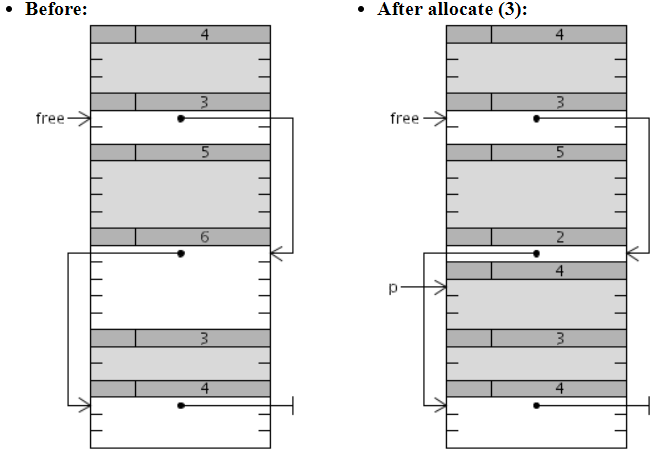
\includegraphics[width=0.8\textwidth]{figures/FF_alg}
    \vspace{-3eX}
    \caption{First fit execution for a request of size 3}
    \label{ff_alg}
    \end{center}
    \vspace{-3eX}
\end{figure}

%first fit algorithm
\begin{algorithm}
\caption{Algorithm for malloc(n)}
\begin{small} 
\begin{algorithmic} 
\REQUIRE $n \geq 0$
\STATE $rsize \leftarrow n + size(header)$  
\STATE Scan free list for first chunk with size $\geq rsize$ 
\IF{chunk not found} 
  \STATE Failure (time for coalescing!) 
\ELSIF{free chunk size is $k \geq rsize + size(header) + 1$} 
   \STATE Split chunk into a free chunk and a busy chunk of size $rsize$
   \STATE Free chunk size $\leftarrow k - rsize$
   \STATE Busy chunk size $\leftarrow rsize$
    \STATE Return pointer to the data part of the Busy chunk 
\ELSE 
    \STATE Unlink chunk from free list 
    \STATE Return pointer to the data part of the chunk 
\ENDIF
\end{algorithmic}
\end{small} 
\end{algorithm}

The main advantage of this method is the fastest search.
The disadvantage, studied in \cite{Knuth73a}, is the localization of the in-use chunks at the start of the heap region.

%best fit algo
\subsubsection{Best-fit method}
The best fit method allocates the free chunk which has the smallest sufficient size.
If such a chunk does not exist, the best fit proceeds like in the failure case of the first-fit method: 
first it tries the coalescing of neighboring free chunks, then it increases the size of the heap region managed.

\begin{figure}[htbp]
    \begin{center}
        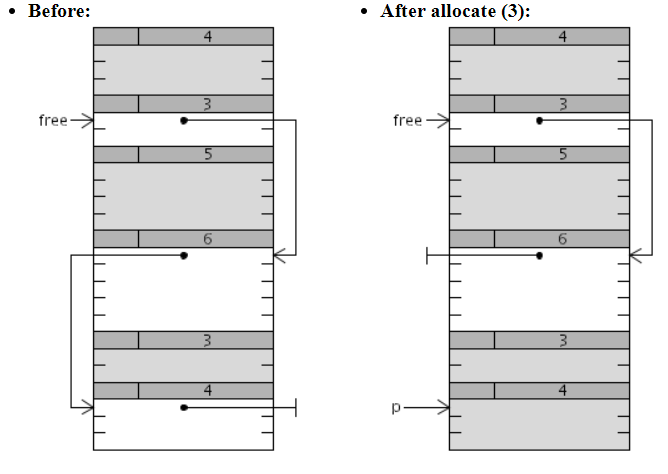
\includegraphics[width=0.8\textwidth]{figures/BF_alg}
    \caption{Best fit execution for a request of size 3}
    \label{bf_alg}
    \end{center}
\end{figure}
%best fit algorithm
\begin{algorithm}
\caption{Algorithm for allocate (n)}
\begin{algorithmic} 
\REQUIRE $n \geq 0$
\REQUIRE $n \geq 0$
\STATE $rsize \leftarrow n + size(header)$  
\STATE Scan free list for for smallest block with size $\geq rsize$ 
\IF{chunk not found} 
  \STATE Failure (time for coalescing!) 
\ELSIF{free chunk size is $k \geq rsize + size(header) + 1$} 
   \STATE Split chunk into a free chunk and a busy chunk of size $rsize$
   \STATE Free chunk size $\leftarrow k - rsize$
   \STATE Busy chunk size $\leftarrow rsize$
    \STATE Return pointer to the data part of the busy chunk 
\ELSE 
    \STATE Unlink chunk from free list 
    \STATE Return pointer to the data part of the chunk 
\ENDIF
\end{algorithmic}
\end{algorithm}


Although best fit minimizes the wastage space, it consumes a lot of time for searching the chunk with smallest size.
 
\subsubsection{Coalescing of free chunks}

Coalescing may be done either at the call of \code{free} (early coalescing allocators) or 
when \code{malloc} does not find a free chunk with enough size (lazy coalescing allocators).

In both cases, the allocator transform the free list by merging in one free chunk two chunks that are neighboring in the heap.


%----------------------------------------------------------------------------------------
%	SECTION
%----------------------------------------------------------------------------------------

\section{Allocators Implemented}
\label{sec:impl}

\subsection{Leslie Aldrige's allocator}
I began first by trying to understand the allocator written by Leslie Aldrige  \cite{Aldridge08} to get an idea about the implementation of allocators. This implementation is based on the first fit method, using a free list.

By testing the code, I've noticed several bugs in his implementation.\marginpar{DETAILS!!!}.
For example, a first problem is ...

I've fixed this problem by ...

The final code is presented in Appendix~\ref{app:leslie}.


\subsection{First version}
This first implementation is based on the first fit method with early coalescing. 
The code is presented in Appendix~\ref{app:first}.

The header has a size field and a next free chunk field, as explained in Section~\ref{sec:impl}.
\begin{lstlisting}[style=cstyle]
typedef struct header
{
  size_t size;			
  struct header *fnx;
} header;
\end{lstlisting}

The field \code{size} is equal to the quotient by the \code{header}'s size (constant \code{BLOCK_SIZE}) of the chunk's size.
Therefore, at allocation, the size requested for the free chunk is obtained by rounding the parameter \code{size} of \code{malloc} to the smallest multiple of \code{header} size (constant \code{BLOCK_SIZE}) plus 1:
\begin{lstlisting}[style=cstyle]
size_t rsize = (size / BLOCK_SIZE + 1) + 1; 
rsize = ((rsize & 1) == 1) ? rsize + 1 : rsize;
\end{lstlisting}

The early coalescing is implemented in \code{free}.
As soon as a chunk is released, checks are made to merge the contiguous free chunks.\marginpar{DETAILS!!!}.

\subsection{Second version}
This second implementation is based on the best fit method with early coalescing. 
The code is presented in Appendix~\ref{app:second}.

The code is very similar to the one of the first version except the scan loop where the best fit is computed.\marginpar{DETAILS!!!}


\subsection{Third version}
This third implementation is based on the first fit method with a free list. 
The code is presented in Appendix~\ref{app:third}.

This version is the same as the first version except that the code of allocation and release has been refactored in several functions (search a chunk, coalescing).
IT IS NOT CLEAR WHAT IS NEW HERE!!\marginpar{DETAILS!!!}


%----------------------------------------------------------------------------------------
%	SECTION
%----------------------------------------------------------------------------------------

\section{Unit Tests for Allocators}
\label{sec:test}
The purpose of unit tests is to verify the expected behavior of a function with respect to a given specification. Here the lack of precise specification forces us to define requirements of these functions, what behaviors are expected or not.

One of the goals of this internship is to conduct a series of tests on the different implementations of the \code{malloc()} and \code{free()} functions. As a result, we will first carry out functional tests and subsequently cover tests (test of instruction and condition, decision or MCDC).
The tests written are included in Appendix~\ref{app:first}.\marginpar{This part is clearly not finished.}

\subsection{Functional tests}

The functional tests consist of a call for each function and the definition of the expected answers. The individual tests will be performed out of any context of use while the test suites will verify a succession of several orders.

\subsubsection{Test of \code{malloc}}
In this test, we try to do some kind of dynamic allocation to make sure that it works properly and then we check that the heap start and the break are not \code{NULL}.

\subsubsection{Test of \code{free}}
In this test, we try to do some dynamic allocation and we release the memory and then we try to see the state of the block to ensure the proper functioning of the function.


\subsection{Coverage tests}

For the coverage tests, we will first perform tests on the functions in individual ways, out of any context of use and those for each of the functions present.
Then we will perform the tests in a context of use with a succession of function call.

\subsubsection{Statement Coverage}
In this test, we try to check all the main lines of the code. We first check that heap start and heap end are \code{NULL} before making an allocation then we check that heap start and heap end are not \code{NULL} and we release the allocated memory.

\subsubsection{MC/DC cover}
In software testing, the modified condition/decision coverage (MC/DC) is a code coverage criterion that requires all of the below during testing:
\begin{enumerate}
\item Each entry and exit point is invoked
\item Each decision takes every possible outcome
\item Each condition in a decision takes every possible outcome
\item Each condition in a decision is shown to independently affect the outcome of the decision.
\end{enumerate}

In this test, I made several malloc and free to make sure that the merge blocks, the algorithm used and all the conditions were respected.


\section{Conclusion}

This internship was an opportunity to revise C programming and the notions learnt during the ``Operating Systems'' course.
In addition, I've learnt how to write unit tests using CUNIT library.
I also learnt how to write documents using \LaTeX.


\bibliographystyle{plain}
\bibliography{bibli}

\newpage
\appendix
\section{Code for Leslie Aldrige's Allocator}
\label{app:leslie}

Here is the revised version of Aldrige's code:

\paragraph{File \code{leslie.h}}
\lstinputlisting[basicstyle=\ttfamily,style=cstyle]{src/lamalloc/leslie.h}

\paragraph{File \code{leslie.c}}
\lstinputlisting[basicstyle=\ttfamily,style=cstyle]{src/lamalloc/leslie.c}

\paragraph{File \code{user_leslie.c}}
\lstinputlisting[basicstyle=\ttfamily,style=cstyle]{src/lamalloc/user_leslie.c}



\section{Code for the first version}
\label{app:first}

\paragraph{File \code{malloc.h}}
\lstinputlisting[basicstyle=\ttfamily,style=cstyle]{src/mbmalloc/FF_malloc/malloc.h}

\paragraph{File \code{malloc.c}}
\lstinputlisting[basicstyle=\ttfamily,style=cstyle]{src/mbmalloc/FF_malloc/malloc.c}

\paragraph{Unit tests}
\lstinputlisting[basicstyle=\ttfamily,style=cstyle]{src/mbmalloc/FF_malloc/main.c}




\section{Code for the second version}
\label{app:second}

\paragraph{File \code{malloc.h}}
\lstinputlisting[basicstyle=\ttfamily,style=cstyle]{src/mbmalloc/BF_malloc/malloc.h}

\paragraph{File \code{malloc.c}}
\lstinputlisting[basicstyle=\ttfamily,style=cstyle]{src/mbmalloc/BF_malloc/malloc.c}

\paragraph{Unit tests}
\lstinputlisting[basicstyle=\ttfamily,style=cstyle]{src/mbmalloc/BF_malloc/main.c}




\section{Code for the third version}
\label{app:third}

\paragraph{File \code{malloc.h}}
\lstinputlisting[basicstyle=\ttfamily,style=cstyle]{src/mbmalloc/freelist_malloc/malloc.h}

\paragraph{File \code{malloc.c}}
\lstinputlisting[basicstyle=\ttfamily,style=cstyle]{src/mbmalloc/freelist_malloc/malloc.c}



\end{document}